\section{Introduction}
% task for experts, large datasources by hand 
%   -> partly automatic would be useful (ranking)
% risk analysis -> relations important
% data required, unstructured i.e. in 10k filings
% where do you get info? newspaper, börse, bankberichte
% what changed? more data. + availability

Evaluating the credibility of a company is an important and complex task for financial experts.
When estimating the risk associated with a potential asset, analysts rely on large amounts of data from a variety of different sources, such as newspapers, stock market trends, and bank statements.
Finding relevant information in mostly unstructured data is a tedious task and examining all sources by hand quickly becomes infeasible.

An important aspect of risk management are the relations of a company of interest to other financial entities.
Automatically extracting such relationships from unstructured text files, such as 10-K filings, significantly reduces the amount of manual work.
Such structured knowledge enables experts to quickly gain insight into a company's relationship network.
However, not all extracted relationships may be important in a given context.
In this paper, we propose an approach to rank extracted relationships based on text snippets, such that important information can be displayed more prominently.
%With our approach we are able to achieve an overall normalized discounted cumulative gain (NDCG) score of 0.98.

% not only for companies relevant -> paper

\section{Dataset}
The dataset used for this work was provided in the context of the FEIII Challenge 2017\cite{feiii_overview}, which contains \emph{triples} extracted from 10-K and 10-Q filings, describing a relationship (\emph{role}) between the \emph{filing company} and a \emph{mentioned financial entity}.
Text snippets of three sentences provide the context a relation appeared in.
%The context a relation appeared in the original filing is given by text snippets of three sentences.
Relationships are limited to ten predefined roles (see \fref{tab:roleresults}).
Judging from their respective text snippets, triples were labelled by experts according to their relevance from a business perspective as \emph{irrelevant}, \emph{neutral}, \emph{relevant}, or \emph{highly relevant}. There are 975 training samples from 25 10-K filings, and 900 triples for testing from 25 disjunct filings.

%Depending on the context, the relevance can be understood as an indicator for the potential impact a relationship might have on the business \textbf{business what? operations?} of the filing company. 

{\setlength{\parindent}{0cm}
\paragraph{\textbf{Task Description}}
The challenge is aimed to explore methods that automatically produce a ranking of triples with the same role by relevance.
This complements last year's challenge to identify financial entities in free text\cite{dsmm16}.
}

{\setlength{\parindent}{0cm}
\paragraph{\textbf{Inter Annotator Agreement}}
The Inter Annotator Agreement, measured by Cohen's Kappa\cite{ir}, has a weighted average of $\overline{\kappa}=0.45$, which indicates a high level of disagreement.
About 40\% of training triples were rated by more than one expert, in the test set all triples received at least three ratings.

%The quality of the annotations is estimated using Cohen's Kappa\cite{ir} ($\kappa\in [0,1]$), which quantifies the inter annotator agreement (IAA) between two experts as shown in \fref{fig:iaa}.
%Around 40\% of the triples were rated by more than one expert with a weighted average of $\overline{\kappa}=0.45$, which indicates a high level of disagreement.
%For our training and evaluation purposes, we map the ratings to numerical values (0--3) and consider the discrete average rating for each triple labelled by multiple experts.
}

%\begin{figure}[b]
%	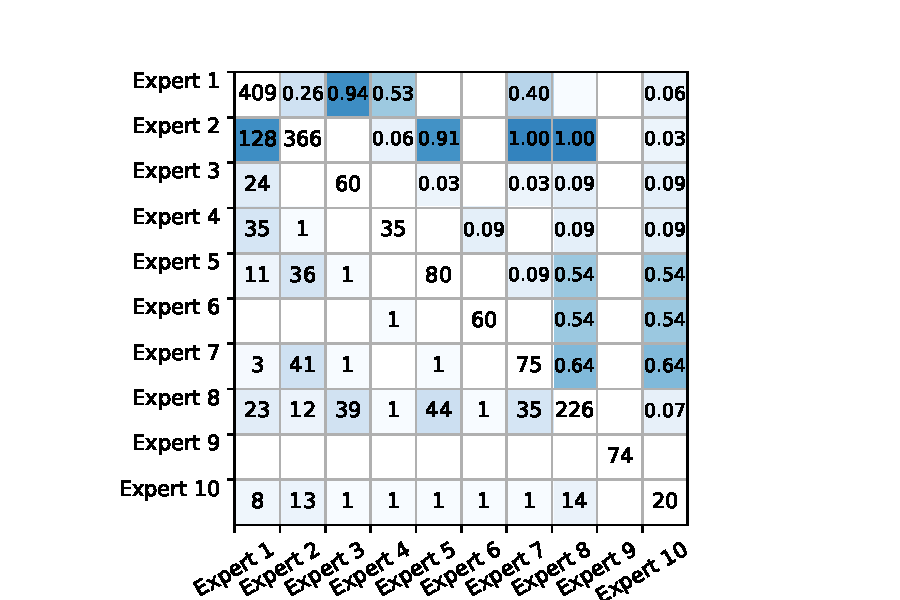
\includegraphics[width=0.8\linewidth]{iaa}
%	\caption{$\kappa$ Inter Annotator Agreement (upper triangular matrix), number of commonly rated triples (lower triangular matrix), and number of ratings (diagonal matrix)}
%	\label{fig:iaa}
%\end{figure}


%{\setlength{\parindent}{0cm}
%\paragraph{\textbf{Additional Data}}
%The triples were extracted from financial documents.
%The surrounding sentences were used by experts to label them.
%Besides the triples, additional information about the word context a triple was extracted from is also given.
%We complement this by the full original filings, which are available online\footnote{\url{https://www.sec.gov/edgar/aboutedgar.htm}}.
%}

\section{Our Approach}
We rank the snippets for each role based on multi-class classifiers, which are trained on the experts' labels.
As input to a classifier we compare three feature sets to represent snippets, namely \emph{bag-of-words} (BOW), \emph{embeddings} (EMB), and \emph{syntax features} (SYN).

We use ensembles of four one-versus-rest Support Vector Classifiers (SVC) with sigmoid kernel, as well as random forests with 20 trees to classify snippets.
The confidence scores in an ensemble are normalised using the softmax function.
From that we derive the ranking score as the maximum probability weighted by its corresponding label.
Class imbalance is adjusted for by weights.

In our experiments, the SVC model has proven to be a good choice for BOW and EMB, but has shown unsatisfactory performances on syntax features.
Therefore, we chose random forests, which perform much better in this case.

Although a model could learn role specific characteristics and improve its performance, we found that due to the limited number of training samples better results are achieved by learning one model from all samples disregarding the role.

%The output probabilities of the classifiers in the ensemble are fed into a softmax function to calculate a weighted ranking score.
%The classifier for BOW and EMB consist of an ensemble of four one-versus-rest logistic regression models, whereas for SYN, a random forest model performs better.
%We apply a softmax function to normalise the ensemble's output. The ranking score is the maximum softmax score weighted by the corresponding label.
 

%We rank the snippets for each role based on an ensemble of multi-class classifiers.
%The ensemble consists of three multi-class classifiers, all trained on different feature sets.
%Two classifier consist of four one-versus-rest logistic regression models trained on the experts' labels.
%The one-versus-rest logistic regression output probabilities of all four classifiers are fed into a softmax function to calculate a weighted ranking score.
%The third classifier is a random forest model.
%The different models of the ensemble are based on different feature sets, namely \emph{bag-of-words} (BOW), \emph{embeddings} (EMB), and \emph{syntax features} (SYN).

% classification model to produce score
% try to learn from labelled data (whats rel/irrel)
% therefore logit
% for features, three approaches
% 3 subsections describing each

\subsection{Bag-of-Words}

Our first model uses a simple bag-of-words representation of the snippets to classify them.
N-grams are extracted for $n=1$ to $3$ and are weighted based on information gain between the classes.
In order to reduce the feature space and guard against over-fitting, the most and least frequent terms are removed from the index.

\begin{table*}[tb]
	\caption{Averaged experimental results for each role using BOW+EMB+SYN}
	\label{tab:roleresults}
	\begin{tabular}{lcccccccccc}
		\toprule
		%    1          2          3           4          5         6        7        8         9           10
		& affiliate & agent & counterpart & guarantor & insurer & issuer & seller & servicer & trustee & underwriter \\
		\midrule %                        1      2      3      4      5      6      7      8      9     10
               \# samples (train/eval) & 185  & 61   & 64   & 34   & 19   & 129  & 20   & 21   & 420  & 21   \\
               \# samples (test)       & 129  & 40   & 108  & 28   & 47   & 98   & 49   & 57   & 304  & 40   \\
               NDCG (5-fold-cv)        & 0.93 & 0.92 & 0.93 & 0.93 & 0.97 & 0.89 & 0.91 & 0.91 & 0.97 & 0.94  \\
               Baseline (random)       & 0.89 & 0.87 & 0.88 & 0.89 & 0.92 & 0.83 & 0.84 & 0.88 & 0.92 & 0.89 \\
		\bottomrule
	\end{tabular}
\end{table*}

\subsection{Sentence Embeddings}
Difficulties with previously unseen examples might arise from the limited training size.
Word embeddings can alleviate this problem by representing words in a 50- to 300-dimensional vector space.
These representations are learned by using unsupervised deep learning.
Internally, a neural network is trained to predict the following word in a sequence of words based on the word's context window. 

We learned paragraph embeddings\footnote{Using Gensim~\url{https://radimrehurek.com/gensim/models/doc2vec.html}} from 25 of the original full text 10-K filing documents containing 60k sentences (2m words).
Previous research has shown, that such embeddings manage to outperform BOW approaches\cite{embeddings}.
We use a window size of 10 and a paragraph vector of size 50, which is trained for 10 epochs over the sentences in all filings.

To build the EMB representation for the text snippet associated with a triple, the embedding is used to induce a vector for each of the three sentences in the snippet, which are then concatenated.
%From the embedding, we induce a vector for each sentence in the text snippet associated with a triple and concatenate them.

\subsection{Syntax Features}
Additionally, to provide a language independent approach, we created a set of syntax-based features.
Following the Gini impurity metric, features, such as the ratio of upper-case words and numbers, or the number of dollar signs and word repetitions, appear to be most meaningful for classification.
In total we chose 20 features describing the amount or presence of different syntactical characteristics.


\subsection{Ensemble}
Each of the numerical representations and their resulting models have individual strengths and weaknesses.
For example, the language independence of SYN can tolerate a changing vocabulary to a certain extent, but misses the advantage to identify key phrases which may prove useful for classification.
As a conclusion, we combined the three models by summing the individual predictions to form a soft vote.

\begin{table}[tb]
	\caption{Experimental results for bag-of-words (BOW), embedding (EMB), syntax (SYN) features, and ensemble}
	\label{tab:results}
	\begin{tabular}{lcccc}
		\toprule
		Approach & NDCG & $\sigma ($NDCG$)$ & F1-Score &  $\sigma ($F1$)$\\
		\midrule
		Baseline (random) & 0.88 & 0.03 & - & - \\
		Baseline (worst)  & 0.72 & 0.06 & - & - \\
		\midrule
		BOW & 0.88 & 0.05 & 0.34 & 0.13\\
		EMB & 0.89 & 0.04 & 0.24 & 0.18\\
		SYN & 0.94 & 0.04 & 0.44 & 0.11 \\
		BOW+EMB+SYN& \textbf{0.95} & 0.04 & 0.43 & 0.12\\
		\bottomrule
	\end{tabular}
\end{table}
%\vfill\null
%\columnbreak
\section{Evaluation}
The system's performance is measured by normalised discounted cumulative gain (NDCG)\cite{ir}.
We perform 5-fold cross-validation \emph{(5-fold-cv)} by leaving out training triples based on the documents they were extracted from. Those triples form the evaluation set \emph{(eval)}.
\Fref{tab:results} lists the mean NDCG scores and the standard deviation ($\sigma$), which are calculated for each role's ranking as shown for the ensemble in \fref{tab:roleresults}.
For comparison, we consider a baseline of the worst possible ranking (inverse order of the ideal ranking) and the average of multiple random rankings.
\newpage
The BOW model performs best on evaluation data (NDCG@0.98) but the feature selection shows seemingly very specific terms which are likely to negatively affect the model's ability to classify unseen samples, which is proven in by the test data.
Training a model on text usually requires a reasonably large corpus which we hope to counteract by using embeddings based on 10-K filings.
However, even the EMB model barely beats the baseline (NDCG@0.92 on eval).
Best and most stable results are achieved with the SYN model and the ensemble, which perform the same on the evaluation data as on test data.

Looking at the performance of the classification task itself (measured by the F1-Score) we observe stable results for the ensemble with low deviation on evaluation data, which is supported by same scores on test data.
Contrary to that is the BOW model, which showed very high deviations and a significant drop from F1-Score 0.73 on evaluation data to test data.

\section{Conclusion}
Overall, we managed to achieve good NDCG scores of around 0.95 using an ensemble of models.
We have shown, that BOW is very sensitive in changing vocabulary used in 10-K filings used in training data to 10-Q filings as in the test data.
Our assumption that paragraph embeddings may be more robust to such changes by training them on a significantly larger set of text and is able to reflect phrase similarities did not hold.
In combination with syntax features in an ensemble, ranking triples describing the relationship between financial entities based on text snippets yields most stable outcomes.

As this work only focuses on a small textual context, for future work we are interested in additional external data, e.g. the impact of a business relationship may be judged by comparing revenues of the involved companies.
Thus, triples could be enriched by adding (historical) revenue of the two involved financial entities. 



%\begin{figure}
%	\begin{subfigure}[t]{0.5\linewidth}
%		\centering
%		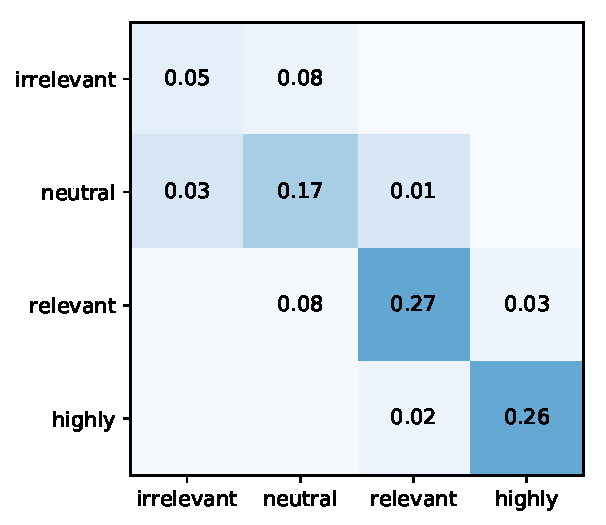
\includegraphics[width=\linewidth]{conf_full}
%		\caption{Trained on all samples}
%	\end{subfigure}%
%	~ 
%	\begin{subfigure}[t]{0.5\linewidth}
%		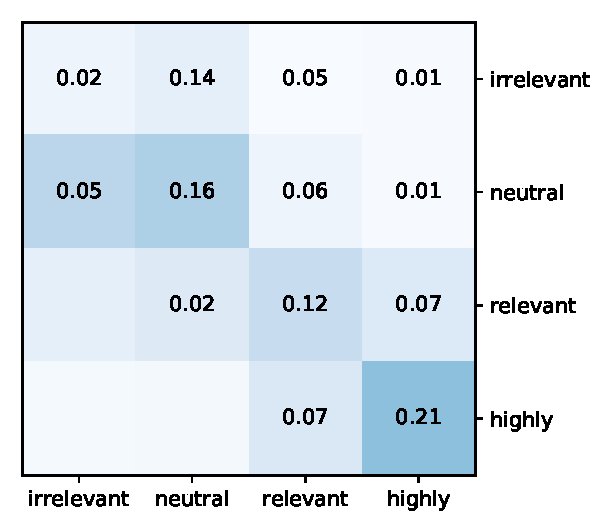
\includegraphics[width=\linewidth]{conf_role}
%		\caption{Trained on role samples}
%	\end{subfigure}
%	\caption{Normalised aggregated confusion matrices for the model with different training sets}
%	\label{fig:confmatrix}
%\end{figure}
%


%\begin{table}
%	\caption{Experimental results for bag-of-words (BOW), embedding (EMB), syntax (SYN) features}, and ensemble (ENS)
%	\label{tab:results}
%	\begin{tabular}{lcc}
%		\toprule
%		Approach & NDCG & $\sigma ($NDCG$)$\\
%		\midrule
%		Baseline (random) & 0.87 & 0.07\\
%		Baseline (worst) & 0.73 & 0.13\\
%		\midrule
%		%F1 full 0.73 std=0.27
%		%F1 role 0.49 std=0.17
%		BOW, full set, categorical & 0.97 & 0.04 \\
%		BOW, role based, categorical & 0.92 & 0.07  \\
%		BOW, full set, continuous & \textbf{0.98} & 0.03 \\
%		BOW, role based, continuous & 0.93 & 0.07 \\
%		\midrule
%		% F1 full 0.41 std=0.16
%		% F1 role 0.38 std=0.21
%		EMB, full set, categorical & 0.91 & 0.07 \\
%		EMB, role based, categorical & 0.89 & 0.07  \\
%		EMB, full set, continuous & 0.92 & 0.07 \\
%		EMB, role based, continuous & 0.90 & 0.08 \\
%		\midrule
%		% F1 full 0.43 std=0.26
%		% F1 role 0.39 std=0.26
%		SYN, full set, categorical & 0.93 & 0.07 \\
%		SYN, role based, categorical & 0.92 & 0.07  \\
%		SYN, full set, continuous & 0.94 & 0.06 \\
%		SYN, role based, continuous & 0.92 & 0.08 \\
%		\midrule
%		% F1 full 0.46 std=0.22
%		% F1 role 0.39 std=0.20
%		ENS, full set, categorical & 0.93 & 0.06 \\
%		ENS, role based, categorical & 0.91 & 0.07  \\
%		ENS, full set, continuous & 0.93 & 0.06 \\
%		ENS, role based, continuous & 0.92 & 0.07 \\
%		\bottomrule
%	\end{tabular}
%\end{table}
